% Chapter Template

\chapter{Evaluations and Discussions} % Main chapter title

\label{Chapter7} % Change X to a consecutive number; for referencing this chapter elsewhere, use \ref{ChapterX}

\lhead{Chapter 7. \emph{Evaluations and Discussions}} % Change X to a consecutive number; this is for the header on each page - perhaps a shortened title

%----------------------------------------------------------------------------------------
%	SECTION 1
%----------------------------------------------------------------------------------------

\section{Evaluations}

The proposed system counts the sheets of cloth by using several image processing techniques. It starts by obtaining an input image from two possible methods, i.e. photographing a new image or choosing from image gallery in the device. It calculates the number of sheets of cloth in the image. The acceptable result has shown on the screen of iPhone device. The screen-shot of the application in case of photographing a new image is shown in Figure \ref{fig:701} and case of selection from image gallery is shown in Figure \ref{fig:f702}.
\begin{figure}[t]
	\centering
	\begin{subfigure}[b]{0.2\textwidth}
		
\includegraphics[width=\textwidth]{f701a.png}
		\caption{}\label{fig:f701a}
	\end{subfigure}
	\begin{subfigure}[b]{0.2\textwidth}
		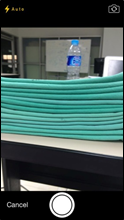
\includegraphics[width=\textwidth]{f701b.png}
		\caption{}\label{fig:f701b}
	\end{subfigure}
	\begin{subfigure}[b]{0.2\textwidth}
		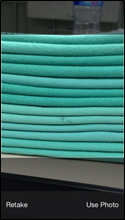
\includegraphics[width=\textwidth]{f701c.png}
		\caption{}\label{fig:f701c}
	\end{subfigure}
	\begin{subfigure}[b]{0.2\textwidth}
		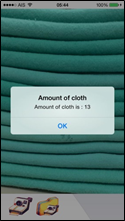
\includegraphics[width=\textwidth]{f701d.png}
		\caption{}\label{fig:f701d}
	\end{subfigure}
	\caption{Screen-shot of sheets of cloth counting application (selecting image file from the gallery)}
	\label{fig:701}
\end{figure}

As shown in Figure \ref{fig:701}, application calculates sheets of cloth from an image taken by device’s built-in camera. The result is shown when user interacts with starting from left to right. Figure \ref{fig:f701a} illustrates the starting screen. There are two icons on the lower left of the screen. The camera icon on the left indicates that the input image is obtained by photographing. The corresponding screen-shot is shown in Figure \ref{fig:f701b}. After obtaining the image, the application asks the user to crop it. This is confirmed when the user presses the “Use Photo” button on the lower right of the screen. This is shown in Figure \ref{fig:f701c}. The application then starts the counting process. The result is reported on a pop-up window as shown in Figure \ref{fig:f701d}. The user can exit from this screen by pressing the “OK” button.
\begin{figure}[t]
	\centering
	\begin{subfigure}[b]{0.2\textwidth}
		
\includegraphics[width=\textwidth]{f702a.png}
		\caption{}\label{fig:f702a}
	\end{subfigure}
	\begin{subfigure}[b]{0.2\textwidth}
		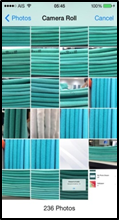
\includegraphics[width=\textwidth]{f702b.png}
		\caption{}\label{fig:f702b}
	\end{subfigure}
	\begin{subfigure}[b]{0.2\textwidth}
		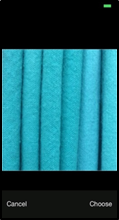
\includegraphics[width=\textwidth]{f702c.png}
		\caption{}\label{fig:f702c}
	\end{subfigure}
	\begin{subfigure}[b]{0.2\textwidth}
		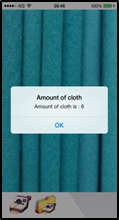
\includegraphics[width=\textwidth]{f702d.png}
		\caption{}\label{fig:f702d}
	\end{subfigure}
	\caption{Screen-shot of sheets of cloth counting application (selecting image file from the gallery)}
	\label{fig:f702}
\end{figure}

As shown in Figure \ref{fig:f702}, application calculates sheets of cloth from an image that is chosen from an image gallery in an iPhone device. The result is shown when user interacts with starting from left to right. Figure \ref{fig:f702a} illustrates the starting screen. There are two icons on the lower right of the screen. The gallery icon on the right indicates that the input image is obtained by choosing from the image gallery. The corresponding screen-shot is shown in Figure \ref{fig:f702b}. After obtaining the image, the application asks the user to crop it. This is confirmed when the user presses the “Choose” button on the lower right of the screen. This is shown in Figure \ref{fig:f702c}. The application then starts the counting process. The result is reported on a pop-up window as shown in Figure \ref{fig:f702d}. The user can exit from this screen by pressing the “OK” button.

\section{Discussions}
The proposed application completes all requirements. And fulfill the aims of counting sheets of cloth with acceptable accuracy comparing to manual count. Thus the application reduces fatigue and time. This application spent a few time to counting sheets of cloth. The result of this project count sheets of cloth is acceptable.